\documentclass[spanish]{beamer}
\usepackage[ansinew]{inputenc} % Acepta caracteres en castellano
\usepackage[spanish]{babel}    % silabea palabras castellanas
\usepackage{amsmath}
\usepackage{mathtools,cancel} % cancela con una flecha \cancelto{0}{XXXX}
\renewcommand{\CancelColor}{\color{red}} %change cancel color to red
\usepackage{amsfonts}
\usepackage{amssymb}
\usepackage{dsfont}
\usepackage{graphicx}
\usepackage{geometry}
\usetheme{Madrid}
\usecolortheme{beaver}
\usepackage{textpos}
% Logo  en el comienzo 
\addtobeamertemplate{frametitle}{}{%
\begin{textblock*}{100mm}(.85\textwidth,-1cm)
{\includegraphics[height=0.4in, keepaspectratio=true]{/Users/luisnunez/Dropbox/MisDocumentos/UIS/UISImagenInstitucional/UISLOGO.png}}
\end{textblock*}}

\begin{document}

\title{\textbf{Potencial efectivo} }
\author[L.A. N��ez]{\textbf{Luis A. N��ez}}  
\institute[UIS]{\textit{Escuela de F�sica, Facultad de Ciencias, } \\
\textit{Universidad Industrial de Santander, Santander, Colombia } \\
{\includegraphics[height=0.4in, keepaspectratio=true]{/Users/luisnunez/Dropbox/MisDocumentos/UIS/UISImagenInstitucional/UISLOGO.png}}
}
\date{\today}
\maketitle


\begin{frame}
\frametitle{Agenda}
  \tableofcontents
\end{frame}


%%%%% Diapo 1
\section{El potencial efectivo}
\frame{
  \frametitle{El potencial efectivo}
   \begin{itemize}  
  	\item<1-> Para el problema de dos cuerpos con un potencial central $V(r)$ 
	$L=\frac{1}{2} \mu\left(\dot{r}^2+r^2 \dot{\theta^2}\right)-V(r) \Rightarrow \frac{d}{d t}\left(\frac{\partial L}{\partial \dot{r}}\right)-\frac{\partial L}{\partial r}=0 \Rightarrow \mu \ddot{r}=-\frac{\partial V}{\partial r}+\frac{l^2}{\mu r^3}$
	\item<2-> La fuerza radial $f(r)=-\frac{\partial V}{\partial r}$ entonces $\mu \ddot{r}=f(r)+\frac{l^2}{\mu r^3} \Rightarrow \mu \ddot{r}=f_{\mathrm{ef}}(r)$
	\item<3-> La fuerza efectiva surge de las contribuciones de la fuerza central $f(r)=-\frac{\partial V}{\partial r}$ y el efecto no inercial $F_{ni} \equiv \frac{l^2}{\mu r^3}=\mu r \dot{\theta}^2$
	\item<4-> Se define una energ�a potencial efectiva, $V_{\mathrm{ef}}(r) \equiv V(r)+\frac{l^2}{2 \mu r^2}$,  tal que $f_{\mathrm{ef}}(r) \equiv-\frac{\partial V_{\mathrm{ef}}}{\partial r}$
	\item<5-> La energ�a total ser� $E  =\frac{1}{2} \mu \dot{r}^2+\frac{l^2}{2 \mu r^2}+V(r)  =\frac{1}{2} \mu \dot{r}^2+V_{\mathrm{ef}}(r)=$ cte.
	\item<6-> Una part�cula de masa $\mu$, movi�ndose en la dimensi�n $r$ con energ�a potencial $V_{\mathrm{ef}}(r)$.
    \end{itemize}
}
%%%%% Diapo 2
\section{Las trayectorias}
\frame{
  \frametitle{Las trayectorias 1/2}
   \begin{itemize}  
  	\item<1-> La condici�n $\dot{r}^2 \geq 0$ implica que este movimento ocurre para valores de $r$ tales que $E \geq V_{\mathrm{ef}}(r)$ 
	\item<2-> Los puntos de retorno est�n dados por la condici�n $\dot{r}=0$, i.e. 
	$E  =V_{\mathrm{ef}}(r)=\frac{l^2}{2 \mu r^2}+V(r)  \Rightarrow E r^2-V(r) r^2-\frac{l^2}{2 \mu}=0$
	\item<3-> Es una ecuaci�n algebraica de segundo grado en $r$ y pueden existir dos ra�ces reales, $r=r_{\min }, r=r_{\max }$. 
	\begin{figure}[t]
		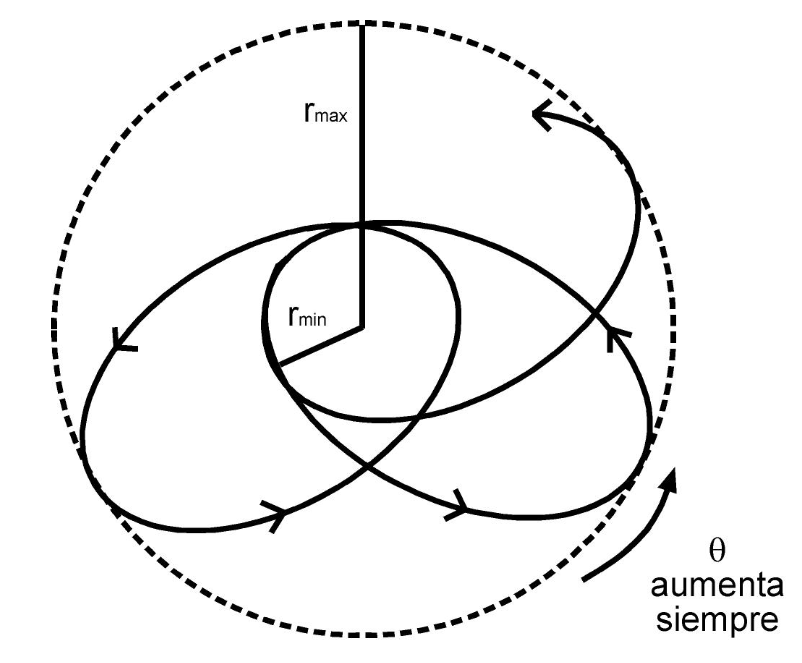
\includegraphics[width=1.5in]{Figuras/Trayectorias.png}
   	\end{figure}
	\begin{itemize}
		\item si $\quad r_{\max }<\infty \quad \Rightarrow$ movimiento es finito, oscilatorio en $r$,
		\item si $\quad r_{\max } \rightarrow \infty \quad \Rightarrow$ movimiento sin retorno,
		\item si $\quad r_{\min }=r_{\max } \quad \Rightarrow$ movimiento es circular.
	\end{itemize}

    \end{itemize}
}
%
% \section{Recapitulando}
\frame{
  \frametitle{Las trayectorias 2/2}
  \begin{enumerate}
	\item<1-> Como $\dot{\theta}=\frac{l}{\mu r^2} \geq 0$, la velocidad angular $\dot{\theta}$ nunca cambia de signo.
	\item<2-> El �ngulo $\theta$ siempre se incrementa en el tiempo y el movimiento siempre ocurre en una misma direcci�n sobre el plano $(r, \theta)$.
	\item<3-> Para encontrar la condici�n de choque $r \rightarrow 0$, i.e. $r_{\min }=0$
	\item<4-> De la ecuaci�n para la energ�a tenemos  
	$\frac{1}{2} \mu \dot{r}^2  =E-V(r)-\frac{l^2}{2 \mu r^2}>0  \Rightarrow E r^2-V(r) r^2-\frac{l^2}{2 \mu}>0$
	\item<5-> Tomando el l�mite $r \rightarrow 0$ tendremos $\lim _{r \rightarrow 0}\left[V(r) r^2\right]<-\frac{l^2}{2 \mu}$
	\item<6-> Consideremos un potencial atractivo de la forma $V(r)=-k / r^n$, entonces $\lim _{r \rightarrow 0}\left[V(r) r^2\right]<-\frac{l^2}{2 \mu} \Rightarrow n>2$
	\begin{itemize}
		\item $V(r)=-k / r^3$ permite caer al centro, $r_{\min }=0$
		\item $V(r)=-k / r^2$, requiere $k>\frac{l^2}{2 \mu}$ para caer al centro de atracci�n
		\item $V(r)=-k / r$ no permite alcanzar $r_{\min }=0$
	\end{itemize} 
  \end{enumerate}
}

  
\end{document}

%%%%% Diapo Fin
\section{Recapitulando}
\frame{
  \frametitle{Recapitulando}
En presentaci�n consideramos
  \begin{enumerate}
  	\item<1->
   \end{enumerate}
}
